\begin{minipage}{0.75\linewidth}
\begin{figure}[h]
    \centering
    \begin{adjustbox}{max width=1.0\linewidth, keepaspectratio}
        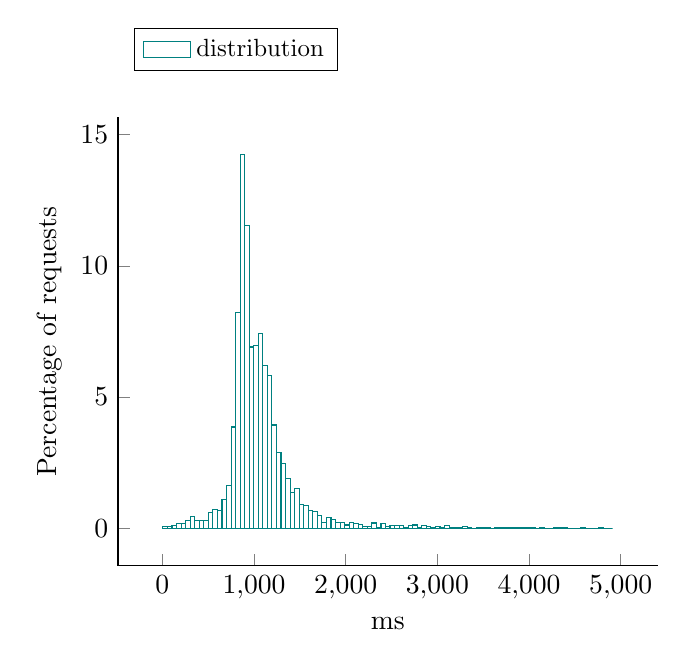
\begin{tikzpicture}
            \begin{axis}[ylabel = Percentage of requests, 
xlabel = ms, 
legend style = {nodes={scale=0.9, transform shape}, at={(0.03,1.2)}, anchor=north west, draw=black, fill=white, align=left, legend columns=3},
area style, mark size = 0pt,
 cycle list name = exotic,
  axis lines* = left]
		\addplot +[ybar interval] coordinates {
			 (6, 0.0625)
			 (55.55, 0.078125)
			 (105.1, 0.109375)
			 (154.65, 0.1875)
			 (204.2, 0.171875)
			 (253.75, 0.28125)
			 (303.3, 0.4375)
			 (352.85, 0.3125)
			 (402.4, 0.28125)
			 (451.95, 0.296875)
			 (501.5, 0.59375)
			 (551.05, 0.71875)
			 (600.6, 0.6875)
			 (650.15, 1.10938)
			 (699.7, 1.625)
			 (749.25, 3.85938)
			 (798.8, 8.21875)
			 (848.35, 14.2344)
			 (897.9, 11.5312)
			 (947.45, 6.90625)
			 (997, 6.95312)
			 (1046.55, 7.40625)
			 (1096.1, 6.21875)
			 (1145.65, 5.82812)
			 (1195.2, 3.9375)
			 (1244.75, 2.89062)
			 (1294.3, 2.46875)
			 (1343.85, 1.90625)
			 (1393.4, 1.35938)
			 (1442.95, 1.51562)
			 (1492.5, 0.890625)
			 (1542.05, 0.875)
			 (1591.6, 0.6875)
			 (1641.15, 0.640625)
			 (1690.7, 0.5)
			 (1740.25, 0.234375)
			 (1789.8, 0.40625)
			 (1839.35, 0.328125)
			 (1888.9, 0.234375)
			 (1938.45, 0.21875)
			 (1988, 0.125)
			 (2037.55, 0.234375)
			 (2087.1, 0.171875)
			 (2136.65, 0.15625)
			 (2186.2, 0.0625)
			 (2235.75, 0.0625)
			 (2285.3, 0.203125)
			 (2334.85, 0.03125)
			 (2384.4, 0.171875)
			 (2433.95, 0.0625)
			 (2483.5, 0.09375)
			 (2533.05, 0.09375)
			 (2582.6, 0.09375)
			 (2632.15, 0.046875)
			 (2681.7, 0.09375)
			 (2731.25, 0.125)
			 (2780.8, 0.015625)
			 (2830.35, 0.09375)
			 (2879.9, 0.0625)
			 (2929.45, 0.015625)
			 (2979, 0.078125)
			 (3028.55, 0.03125)
			 (3078.1, 0.109375)
			 (3127.65, 0.03125)
			 (3177.2, 0.03125)
			 (3226.75, 0.03125)
			 (3276.3, 0.0625)
			 (3325.85, 0.015625)
			 (3375.4, 0)
			 (3424.95, 0.015625)
			 (3474.5, 0.015625)
			 (3524.05, 0.015625)
			 (3573.6, 0)
			 (3623.15, 0.015625)
			 (3672.7, 0.015625)
			 (3722.25, 0.03125)
			 (3771.8, 0.015625)
			 (3821.35, 0.015625)
			 (3870.9, 0.046875)
			 (3920.45, 0.015625)
			 (3970, 0.015625)
			 (4019.55, 0.015625)
			 (4069.1, 0)
			 (4118.65, 0.03125)
			 (4168.2, 0)
			 (4217.75, 0)
			 (4267.3, 0.03125)
			 (4316.85, 0.03125)
			 (4366.4, 0.015625)
			 (4415.95, 0)
			 (4465.5, 0)
			 (4515.05, 0)
			 (4564.6, 0.015625)
			 (4614.15, 0)
			 (4663.7, 0)
			 (4713.25, 0)
			 (4762.8, 0.015625)
			 (4812.35, 0)
			 (4861.9, 0)
			 (4911.45, 0)
		};
\addlegendentry{distribution};
           \end{axis}
      \end{tikzpicture}
  \end{adjustbox}
  \caption{Response time distribution - req = ReadTimeline-3}
\end{figure}
\end{minipage}\hfill\begin{minipage}{0.18\linewidth}
\begin{table}[h]
\begin{tabular}{|cc|}
\hline
\textbf{} & \textbf{ms}\\ \hline
 \Xhline{0.005\arrayrulewidth}
min & 6\\
 \Xhline{0.005\arrayrulewidth}
max & 4961\\
 \Xhline{0.005\arrayrulewidth}
mean & 1066\\
 \Xhline{0.005\arrayrulewidth}
std & 394\\
\hline
\hline
 \Xhline{0.005\arrayrulewidth}
25th & 872\\
 \Xhline{0.005\arrayrulewidth}
50th & 985\\
 \Xhline{0.005\arrayrulewidth}
75th & 1166\\
 \Xhline{0.005\arrayrulewidth}
80th & 1217\\
 \Xhline{0.005\arrayrulewidth}
85th & 1295\\
 \Xhline{0.005\arrayrulewidth}
90th & 1415\\
 \Xhline{0.005\arrayrulewidth}
95th & 1660\\
 \Xhline{0.005\arrayrulewidth}
99th & 2779\\
\hline
\end{tabular}
\caption{Response time}
\end{table}
\end{minipage}\hfill